\documentclass[10pt,a4paper,notitlepage]{article}
\usepackage[utf8]{inputenc}
\usepackage[T1]{fontenc}
\usepackage{amsmath}
\usepackage{amsfonts}
\usepackage{amssymb}
\usepackage{array}
\usepackage{float}
\usepackage{graphicx}
\usepackage{subcaption}
\usepackage{float}
\usepackage{bm}
\begin{document}
\title{Project CFD--Lab\\ \textit{Free Surface Simulation}}
\author{\textbf{Group Number: 1}\\Ioannis Kouroudis, Lukas Krenz, Andreas Reiser,  \\ \\\textbf{Supervisor}\\Friedrich Menhorn}
\maketitle
\section*{Abstract}
In industry there are many applications that require the simulation of a system of unmixable fluids with vastly different kinematic viscosity, separated by a discrete interface.  This problem is commonly referred to as a free surface flow problem. In effect, the kinematic viscosity difference causes the first fluid, which is usually the industrially relevant one, to exert force on the second one, receiving a negligible reaction in return. The most common configuration of this sort is a liquid-gas system and is frequently encountered in applications such as dam breaking scenarios, material processes and wave simulations.
In this particular project, the phenomenon is simulated  using a Lattice Boltzmann approach combined with a volume of fluid method.
        
\section{Implementation \textit{\&} Theory}
The algorithm generally works by keeping track of the mass exchange between cells.
To do this, we save the mass $m$ for each cell and convert the cells if they are either full or empty.
Between the filled and empty cells we insert interface cells.
The program was written in C\texttt{++} utilising OpenMP parallelization.
We followed the algorithm described in~\cite{thurey2007physically}.

\subsection{Gravity }
We modify the standard collision process to include the gravity force $\bm{g}$~\cite{thurey2006optimization}
\begin{equation}\label{eq:BGK}
f_{i}^*(\bm{x},t) =f_i (\bm{x}, t) - \frac{1}{\tau} \left( f_i(\bm{x}, t) - f_{i}^{eq}\rho(\bm{x},t),\mathbf{u}(\bm{x},t)+\tau \bm{g}) \right).
%f_{i}(x,t+\Delta t)=(1-\omega)f_{i}^{eq}+\omega f_{i}^{eq}(\rho(\mathbf{x},t),\mathbf{u}(\mathbf{x},t)+\frac{\bm{g}}{\omega}).
\end{equation}

\subsection{Mass exchange}
In order to keep track of the interface, two additional variables have to be stored for each cell, namely the mass $m$ and the fluid fraction $\varepsilon_i = \frac{m_{i}}{\rho_{i}}$.
The mass exchanged between an interface and a fluid cell can be calculated directly using their distributions
\begin{equation} \label{eq:fluid-interface}
\Delta m_{i}(\bm{x},t)=f_{\hat{i}}(\bm{x}+\bm{e}_{i},t)-f_{i}(\bm{x},t),
\end{equation}
where $\hat{i}$ is the inverse velocity of $i$.
The interface--interface mass exchange
\begin{equation} \label{eq:intint}
\Delta m_{i}(\bm{x},t+\Delta t)=s_{e} \frac{\varepsilon(\bm{x}+\Delta t \bm{e}_{i},t)+\varepsilon(\bm{x},t)}{2}
\end{equation}
takes the fluid fraction of both cells into account.
To avoid ``lonely'' interface cells that have no empty or filled neighbours, we use the appropriate \(s_e\) from table \ref{table:artifacts} in equation \eqref{eq:intint}.
Because the mass exchange is a symmetric process, the used scheme is explicitly mass preserving.

\begin{table}[ht]
\centering
\hspace*{-2cm} % dirty hack to centre table
\begin{tabular}{lllll}
 		&  standard cell at $(\bm{x}+e_{i})$	& no fluid nb at $(\bm{x}+\bm{e}_{i})$     & no empty nb at $(\bm{x}+\bm{e}_{i})$    \\
 standard cell at $(\bm{x})$		&$f_{\hat{i}}(\bm{x}_{nb},t)-f(\bm{x},t)$	&  $f_{\hat{i}}(\bm{x}_{nb},t)$		&$-f_{i}(\bm{x},t)$		    \\
 no fluid neighbours at $(\bm{x})$	&$-f_{i}(\bm{x},t)$			&  $f_{\hat{i}}(\bm{x}_{nb},t)-f(\bm{x},t)$	&$-f_{i}(\bm{x},t)$		     \\
 no empty neighbours at $(\bm{x})$	&$f_{\hat{i}}(\bm{x}_{nb},t)$	&  $f_{\hat{i}}(\bm{x}_{nb},t)$		&$f_{\hat{i}}(\bm{x}_{nb},t)-f(\bm{x},t)$
\end{tabular}
\caption{\label{table:artifacts}Interface--Interface mass streaming coefficient $s_{e}$ with $x_b$ as the neighbouring cell.}
\end{table}

\subsection{Boundary conditions}
Because interface cells have empty cells as neighbours, they do not have a full set of distributions.
This is why we need to reconstruct all distributions coming from empty cells during the streaming step.
The physical perspective of this condition is that the gas has a far greater kinematic viscosity and is consequently pushed without resistance by the liquid.
Furthermore we use the atmospheric pressure ($\rho_{A} = 1$) in place of the density in the equilibrium function.
If $\bm{e}_{i}$ comes from an empty cell into a interface cell the following distribution is constructed:
\begin{equation} \label{eq:dist}
f'_{\hat{i}} (\bm{x}, t + \Delta t) = f^{eq}_{\hat{i}}(\rho_A, \mathbf{u})+f^{eq}_{{i}}(\rho_A, \mathbf{u})-f_{i}(\mathbf{x},t).
\end{equation}

However, constructing these distributions along only one side of the interface would result in a force imbalance.
To rectify this, we additionally reconstruct distributions coming in along the surface normal, which we approximate by central differences
\begin{equation} \label{eq:normal}
  \mathbf{n}=\frac{1}{2}\begin{bmatrix} \varepsilon(x_{j-1,k,l})-\varepsilon(x_{j+1,k,l})\\\varepsilon(x_{j,k-1,l})-\varepsilon(x_{j,k+1,l})
    \\
    \varepsilon(x_{j,k,l-1})-\varepsilon(x_{j,k,l+1} ) \end{bmatrix},
\end{equation}
where $\varepsilon(x_{j,k,l})$ is the fluid fraction of the cell at coordinates $(j,k,l)$.
If $\mathbf(\bm{n} \cdot \bm{e_i})>0$, $f_{i}$ is reconstructed according to equation \eqref{eq:dist}


\subsection{Flag Update}
After the mass calculation step, all interface cells that have filled or emptied are assigned temporary flag as filled or emptied cells respectively.
To determine this, the criterion
\begin{equation} \label{eq:filled}
m(\bm{x},t+ \Delta t)>(1+ \text{offset }) \cdot \rho(\bm{x},t+\Delta t),
\end{equation}
\begin{equation} \label{eq:empty}
m(\bm{x},t+ \Delta t)<(0- \text{offset }) \cdot \rho(\bm{x},t+\Delta t),
\end{equation}
is used, with an offset of $10^{-3}$, to avoid oscillating changes of the cell status~\cite{thurey2007physically}.

We then convert all empty neighbours of filled cells to interface cells and all neighbouring emptied cells back to interface cells.
After this is done, all fluid neighbours of emptied cells are converted to interface cells.
Formerly empty cells that became interface cells are initialised with the average density and velocity of their fluid, interface and filled neighbours.
We need to use temporary flags because otherwise the update rule would be order dependent.

\subsection{Excess Mass }
Newly converted cells have an excess mass $m^{\text{ex}}$.
Fluid cells should have mass equal to their density, empty cells should have mass zero.
All excess mass is distributed to all interface neighbours.
For reasons of stability, we weigh the updates according to the position of the current interface
\begin{equation} \label{eq:exmass}
\Delta m(\bm{x}+\bm{e}_{i})=m^{\text{ex}}\frac{v_{i}}{v_{\text{total}}},
\end{equation}
where $v_{i}$ is the weight of the neighbouring cell and $v_{\text{total}}$ is the sum of all weights.
The weights are calculated by
\begin{align}
  \label{eq:excessMassWeights}
 v_i^f &=  \max(0, \bm{n} \cdot \bm{e_i}),\\
 v_i^e &= - \min(0, \bm{n} \cdot \bm{e_i}),
\end{align}
for filled and emptied cells respectively.

Again it is important to update the mass of all cells at the same time.
After the excess mass has been distributed, all flags are converted from the temporary to the finalised ones.

\subsection{Adaptive time step \textit{\&} turbulence model}
If velocities become larger than $1/3$ distributions can become negative thus impacting the stability.
To avoid instabilities due to high velocities and to acquire speedup during periods of rest we use an adaptive time step.
We use a critical velocity of $\bm{u_\text{crit}} = 1/6$, which is half the lattice speed of sound.

To adapt the time step, we calculate the maximum velocity $\bm{u}_{\text{max}}$ of the simulation and modify the time step if needed.
If $ \Vert \bm{u}_{max} \Vert > \xi \bm{u}_{\text{crit}}$ the new timestep becomes $\Delta t_{\text{new}}= \xi \Delta t_{\text{old}}$ and if 
$\Vert \bm{u}_{max} \Vert < \xi \bm{u}_\text{crit}$ the new timestep is updated to $\Delta t_{\text{new}} = \Delta t_{\text{old}} / \xi$,
where $\xi = 4/5$ is the rescaling factor~\cite{thurey2005interactive}.
The timestep is used to compute a new value of the relaxation parameter $\tau$
\begin{equation} \label{eq:omega}
\tau_{\text{new}}= \frac{\Delta t_{\text{new}}}{\Delta t_{\text{old}}} (\tau_{\text{old}}- 0.5) +0.5
\end{equation}
which is then used in the collision process.

After each time step change, all time dependent values must be rescaled, e.g.~density, mass, velocity and gravity.
Additionally all distributions must be rescaled.
The details of the rescaling procedure are omitted to preserve space, the interested reader is referred to chapter 6 of~\cite{thurey2007physically}.

For very small time steps or viscosities, $\tau$ is close to $0.5$, thus leading to instabilities in the simulation.
To rectify this, we use a Smagorinsky turbulence model.
For this we calculate the local stress tensor $S$ by
\begin{equation} \label{eq:stress}
\Pi_{\alpha,\beta}=\sum^{19}_{i=1}e_{i\alpha}e_{i\beta}(f_{i}-f_{i}^{eq}),
\end{equation}
where $\alpha$ and $\beta$ are the components of the lattice velocities.
 The intensity $S$ is then given by 
\begin{equation} \label{eq:intensity}
S=\frac{1}{6C^{2}}(\sqrt{\nu^{2}+18C^{2}\sqrt{\Pi_{\alpha,\beta} \Pi_{\alpha,\beta}}-\nu},
\end{equation}
where summation over $\alpha$ and $\beta$ is implied and $C$ is a constant usually set to values close to $0.03$~\cite{thurey2007physically}.
Finally we set the local relaxation time to
\begin{equation} \label{eq:relax}
\tau_s=3(\nu+C^{2}S)+\frac{1}{2},
\end{equation}
where $\nu$ is the global viscosity.
Intuitively, the turbulence model increases the local viscosity for cells according to the stress exerted onto them.

\section{Results \textit{\&} Scenarios}
Two simple scenarios were chosen which produced both physically correct and visually pleasing results.
\subsection{Dam Breaking}
The dam breaking was simulated by a large vertical mass of fluid that is released and affected by gravity.
\begin{figure}[H]
\centering
\begin{subfigure}{0.25\textwidth}
  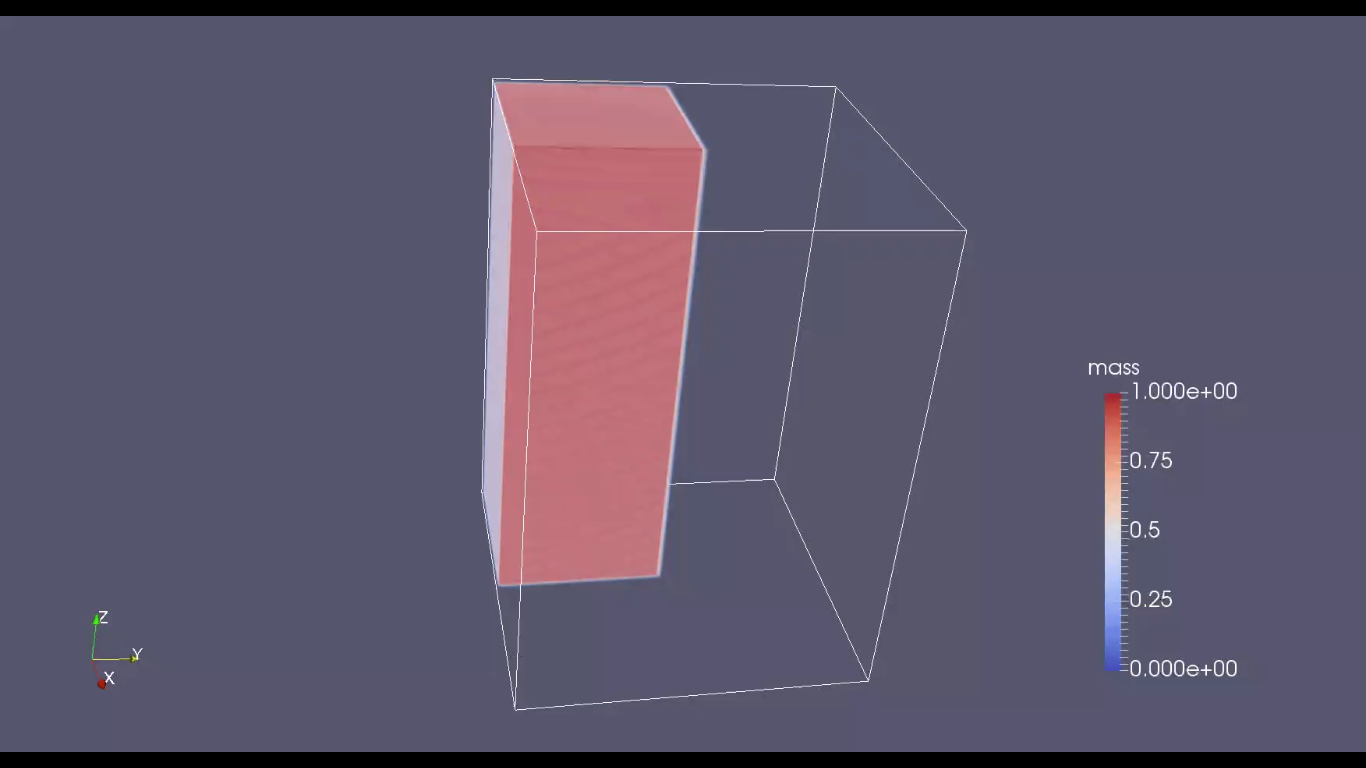
\includegraphics[width=1.0\linewidth]{dam/1.png}
\end{subfigure}%
\begin{subfigure}{0.25\textwidth}
  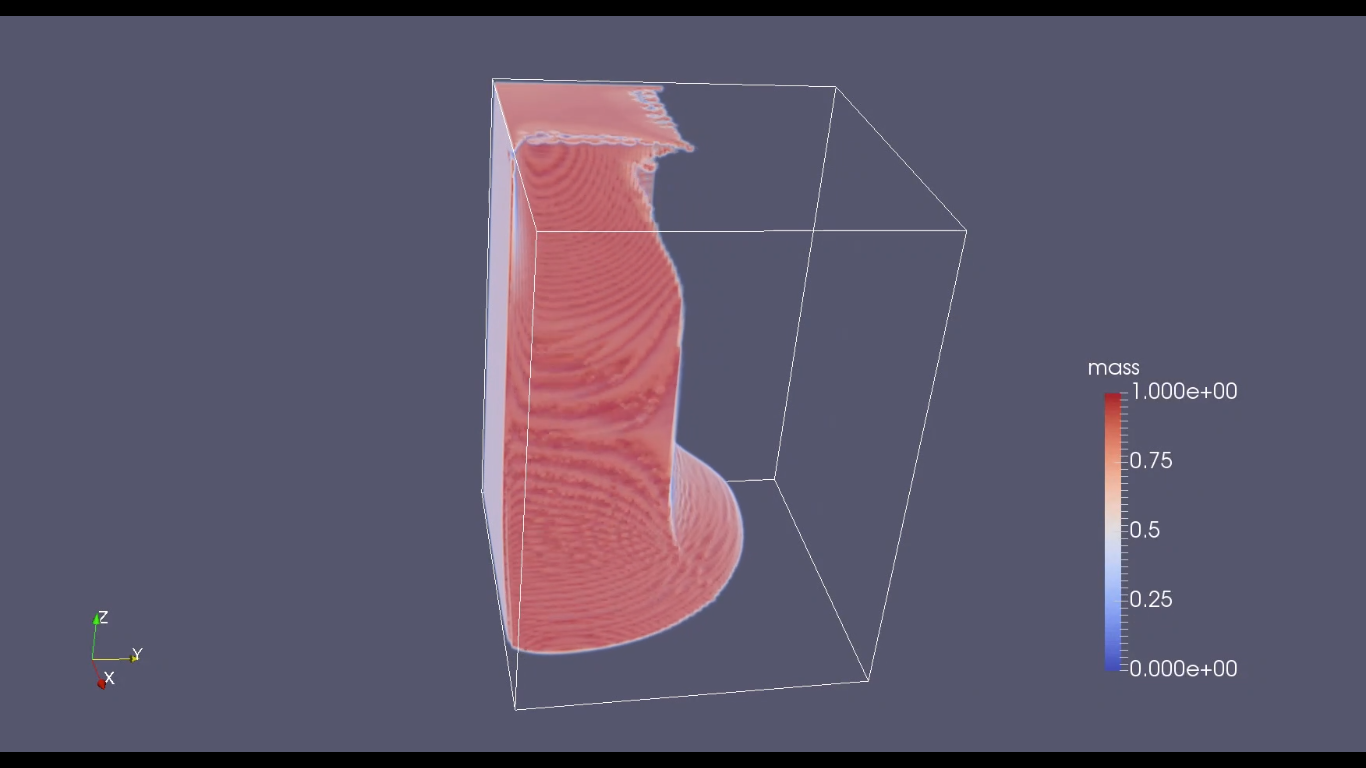
\includegraphics[width=1.0\linewidth]{dam/2.png}
\end{subfigure}
\begin{subfigure}{0.25\textwidth}
  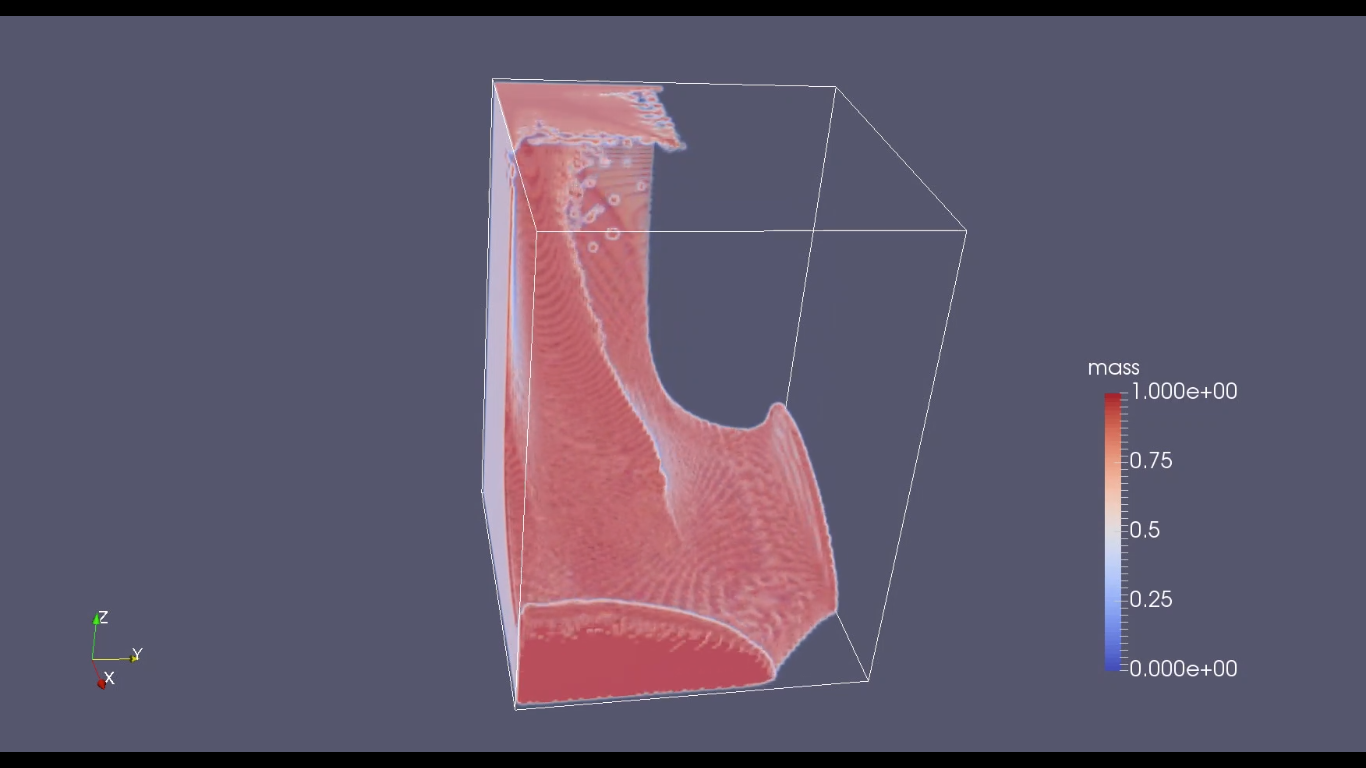
\includegraphics[width=1.0\linewidth]{dam/3.png}
\end{subfigure}
\centering
\begin{subfigure}{0.25\textwidth}
  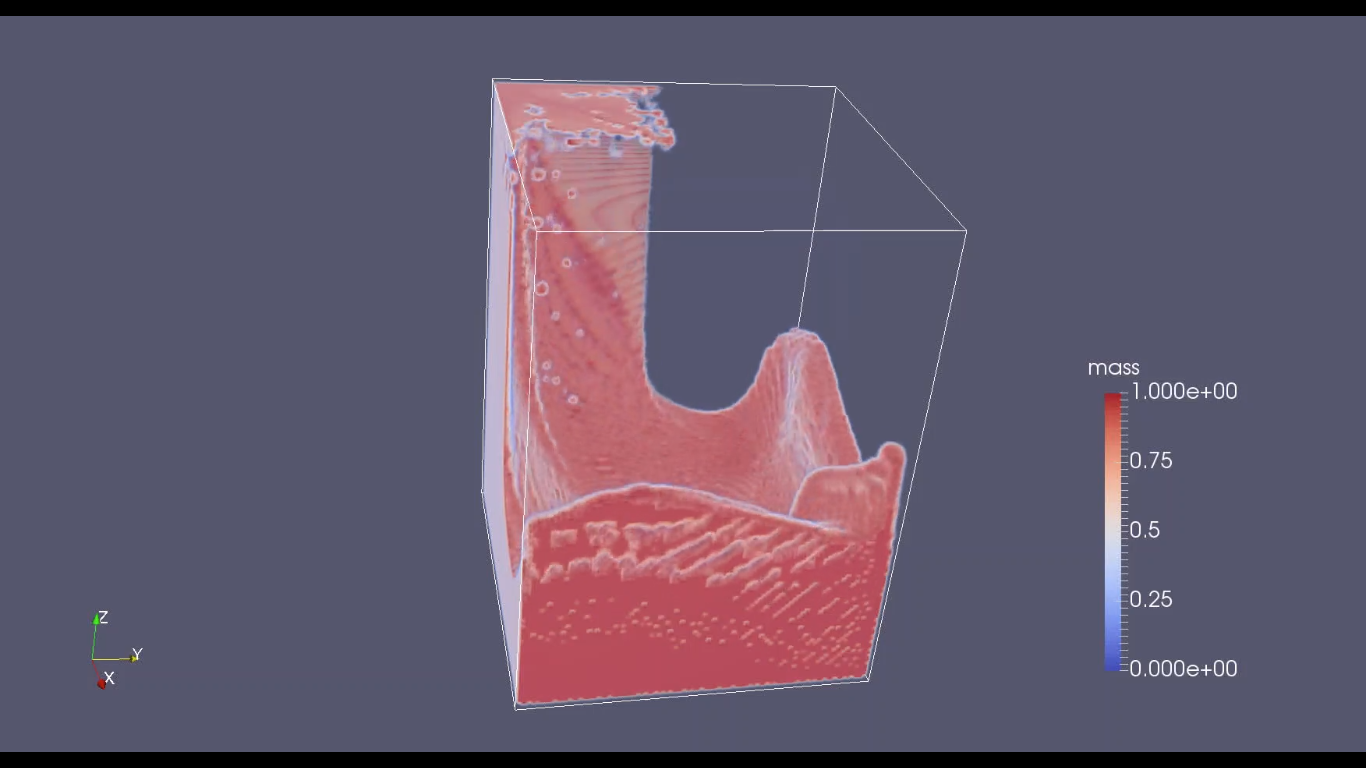
\includegraphics[width=1.0\linewidth]{dam/4.png}
\end{subfigure}%
\begin{subfigure}{0.25\textwidth}
  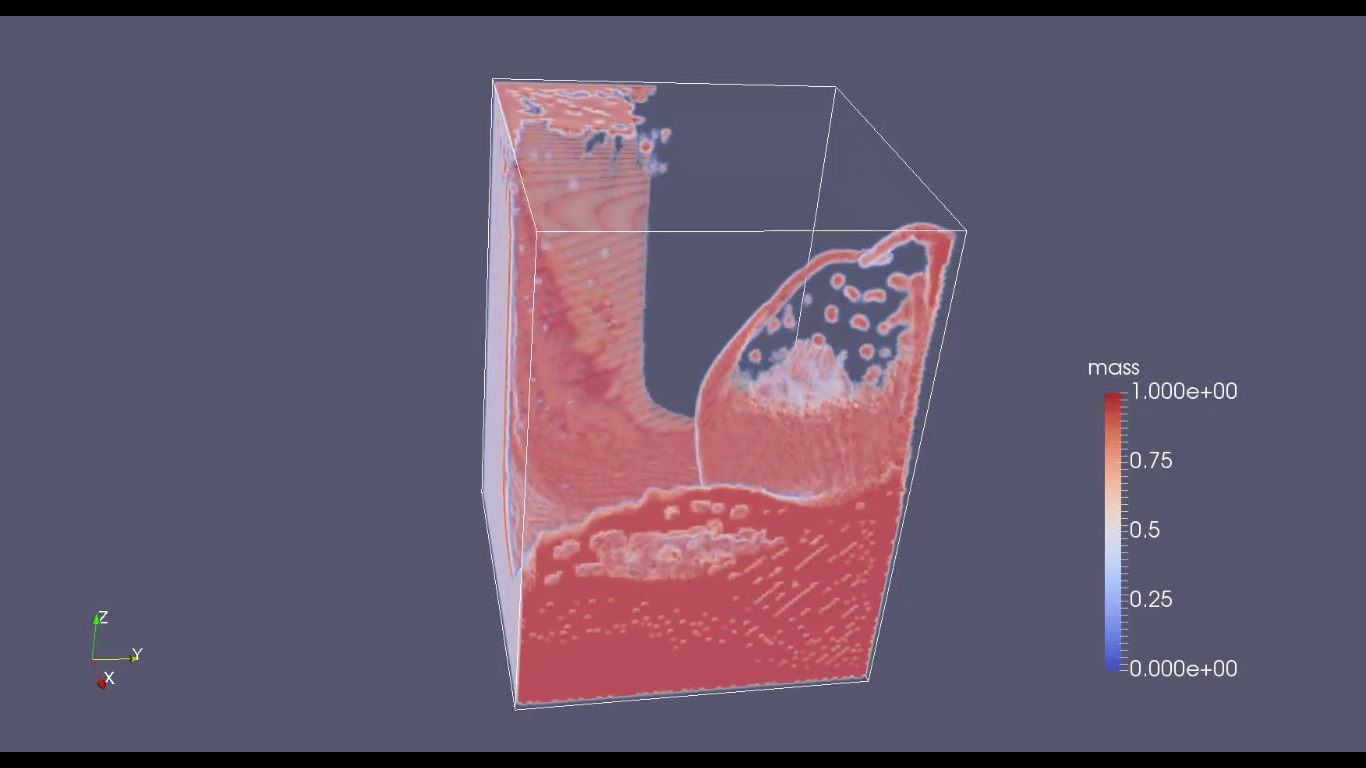
\includegraphics[width=1.0\linewidth]{dam/5.png}
\end{subfigure}
\begin{subfigure}{0.25\textwidth}
  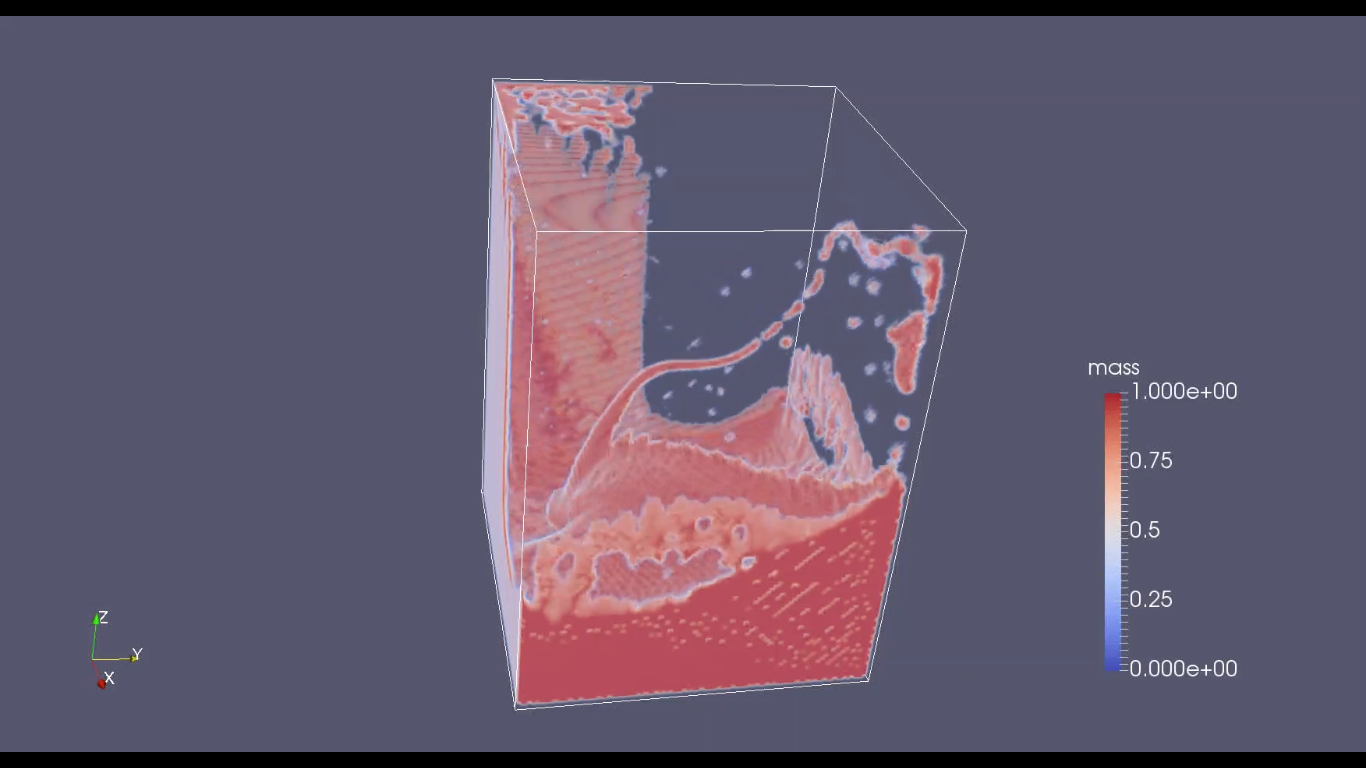
\includegraphics[width=1.0\linewidth]{dam/6.png}
\end{subfigure}
\centering
\begin{subfigure}{0.25\textwidth}
  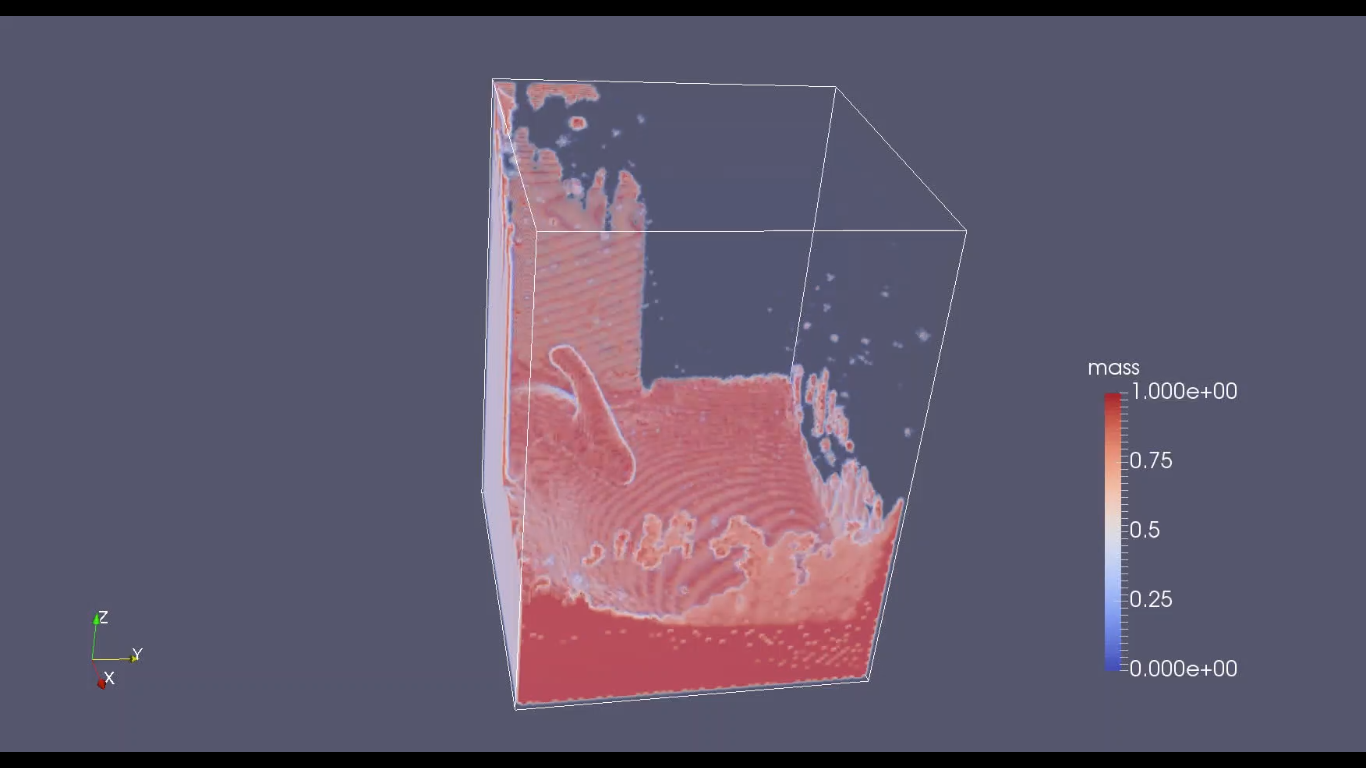
\includegraphics[width=1.0\linewidth]{dam/7.png}
\end{subfigure}%
\begin{subfigure}{0.25\textwidth}
  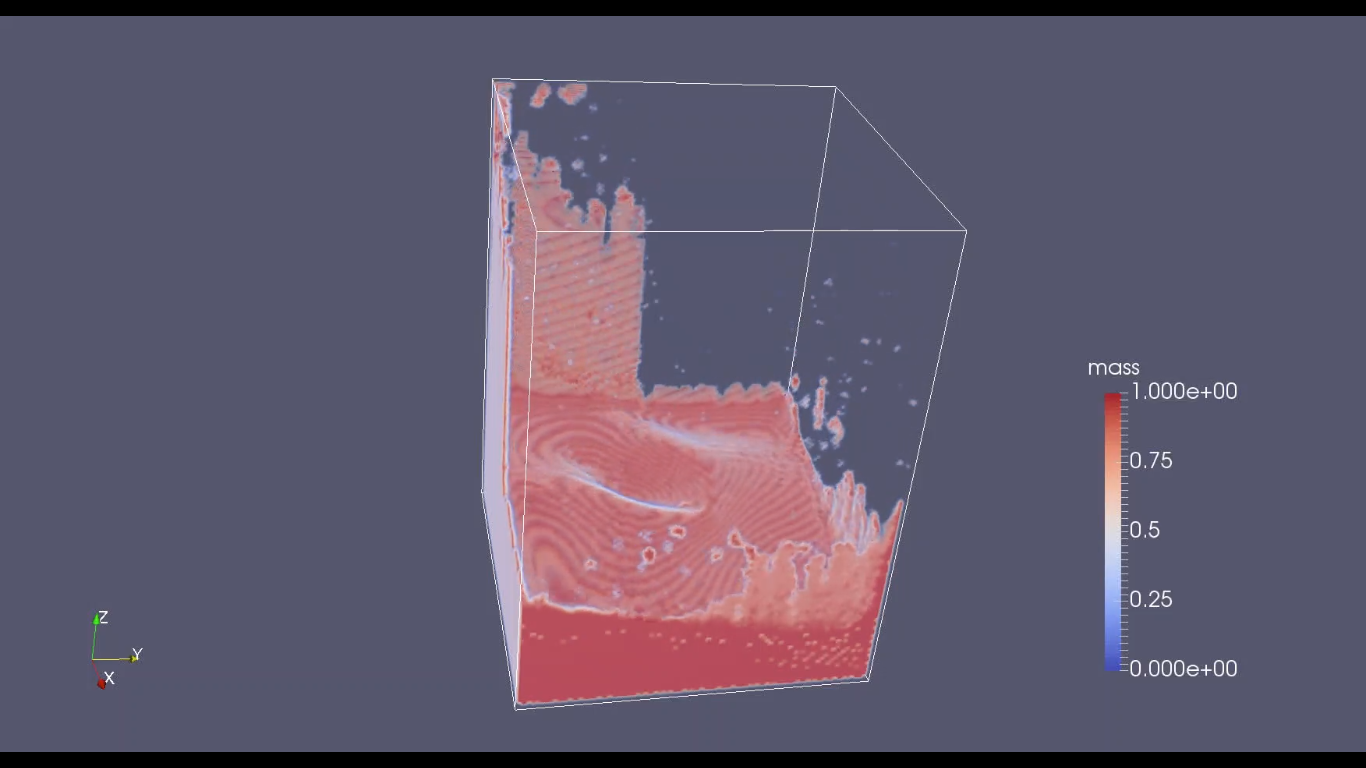
\includegraphics[width=1.0\linewidth]{dam/8.png}
\end{subfigure}
\begin{subfigure}{0.25\textwidth}
  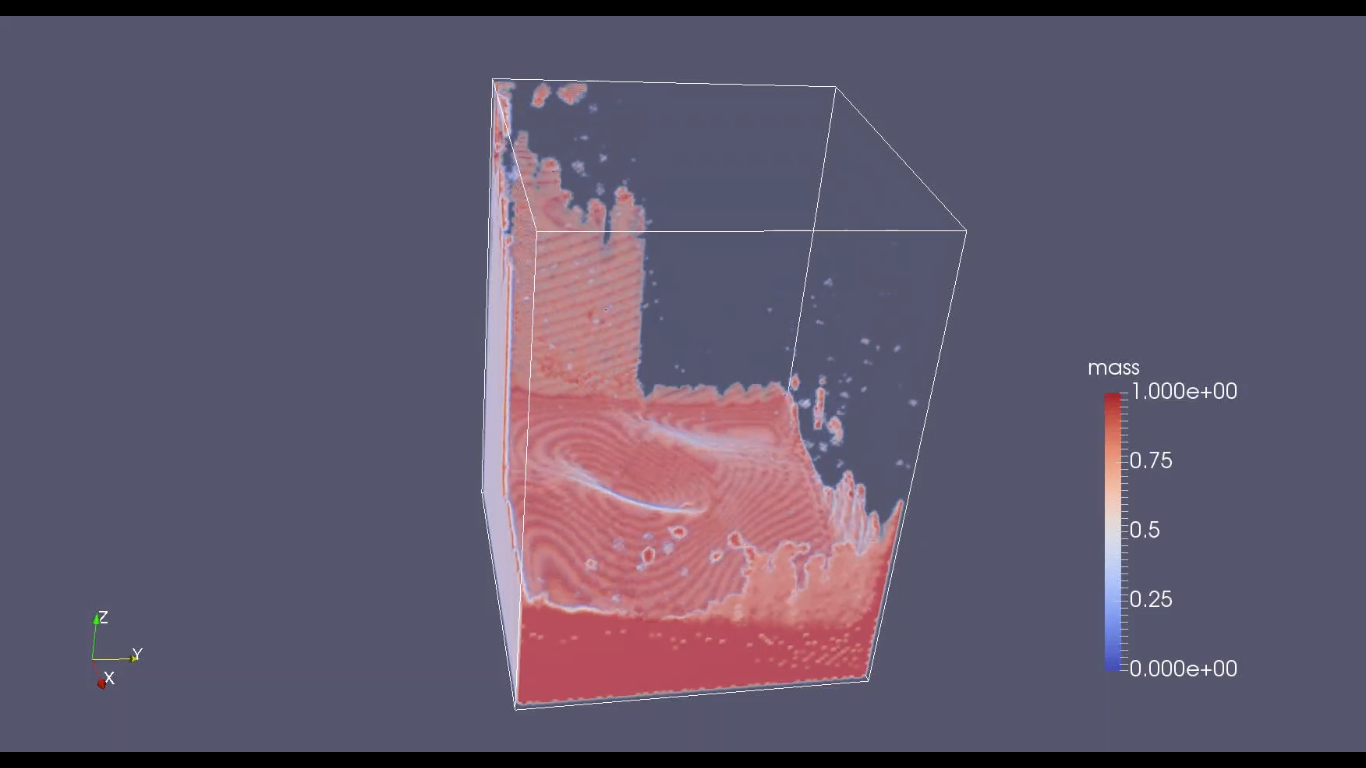
\includegraphics[width=1.0\linewidth]{dam/9.png}
\end{subfigure}
\caption{Breaking Dam}
\label{fig:dam}
\end{figure}
\subsection{Falling Drop}
A drop was left to fall in a pool of stationary water. The results look comparable to other sources and resemble the expected physical behaviour.
\begin{figure}[H]
\centering
\begin{subfigure}{0.25\textwidth}
  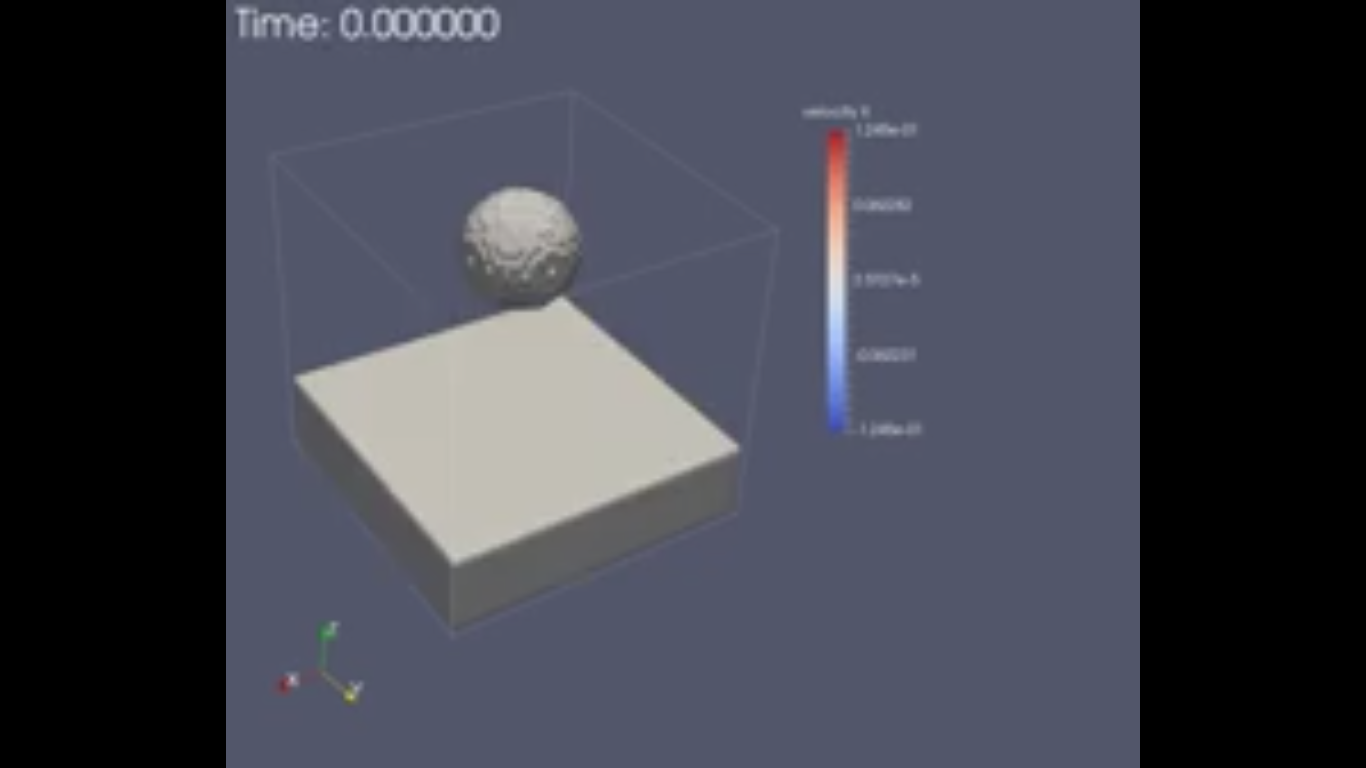
\includegraphics[width=1.0\linewidth]{drop/1.png}
\end{subfigure}%
\begin{subfigure}{0.25\textwidth}
  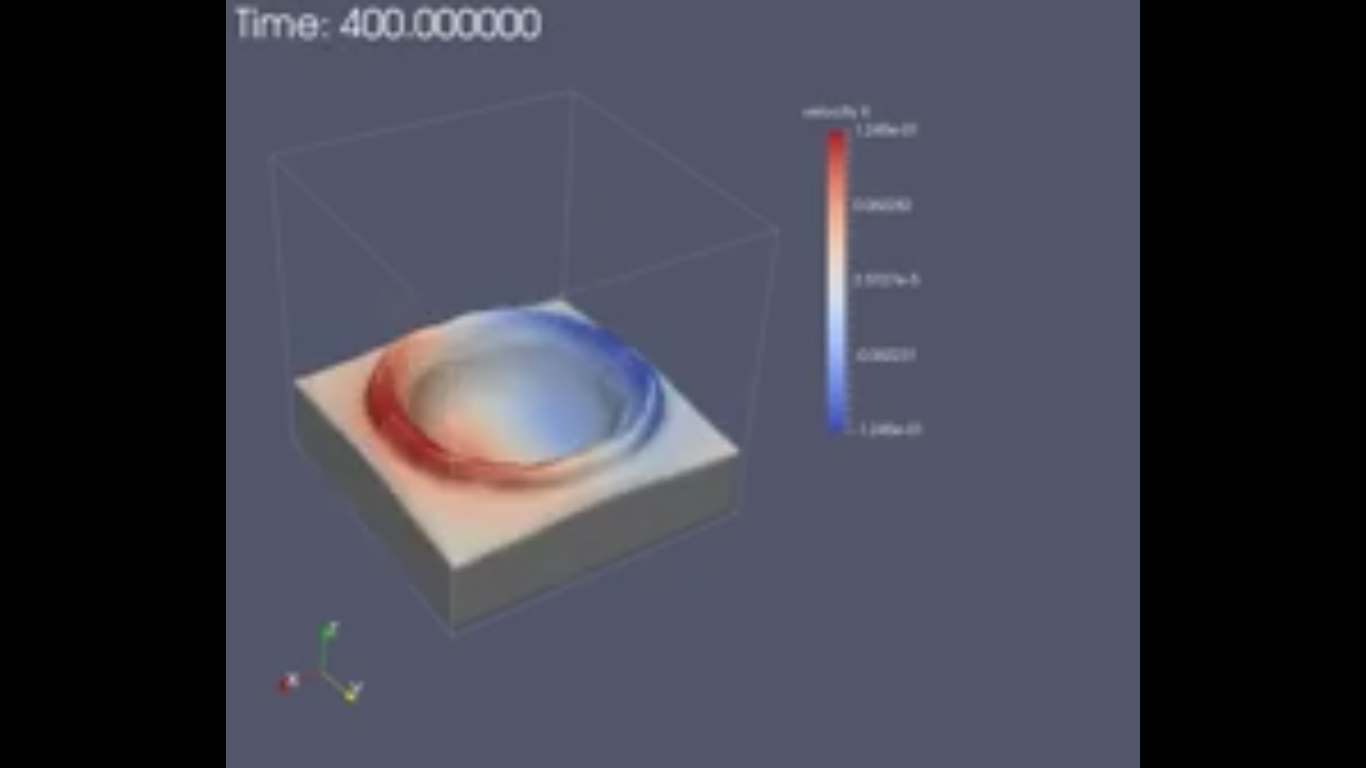
\includegraphics[width=1.0\linewidth]{drop/2.png}
\end{subfigure}
\begin{subfigure}{0.25\textwidth}
  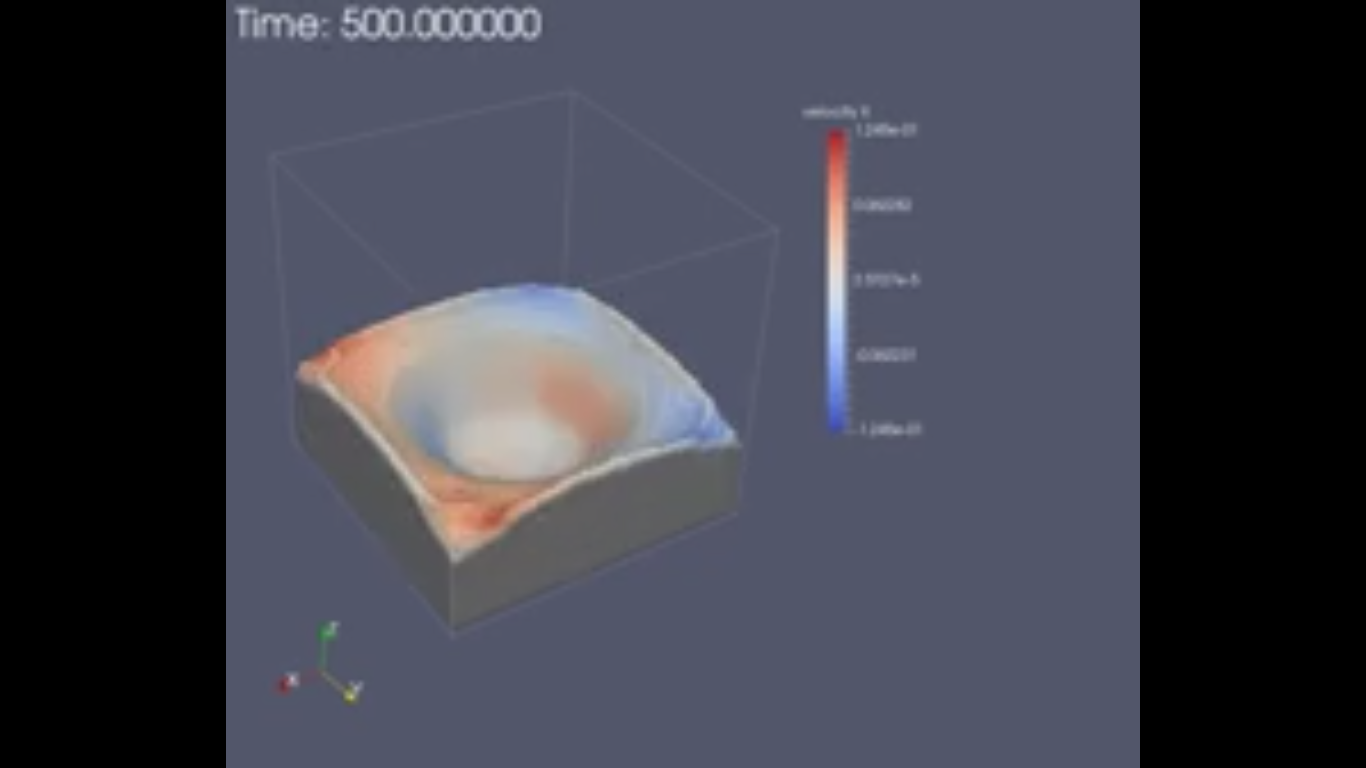
\includegraphics[width=1.0\linewidth]{drop/3.png}
\end{subfigure}
\centering
\begin{subfigure}{0.25\textwidth}
  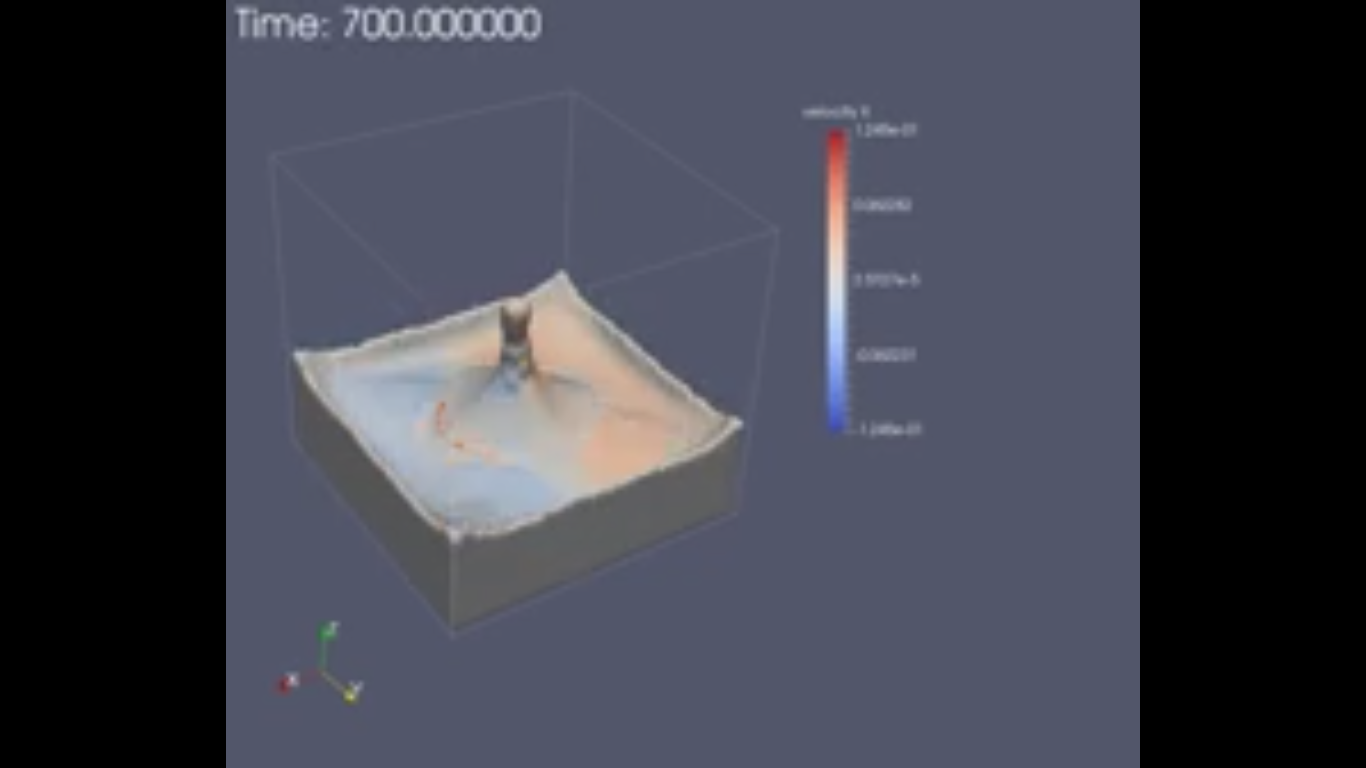
\includegraphics[width=1.0\linewidth]{drop/4.png}
\end{subfigure}%
\begin{subfigure}{0.25\textwidth}
  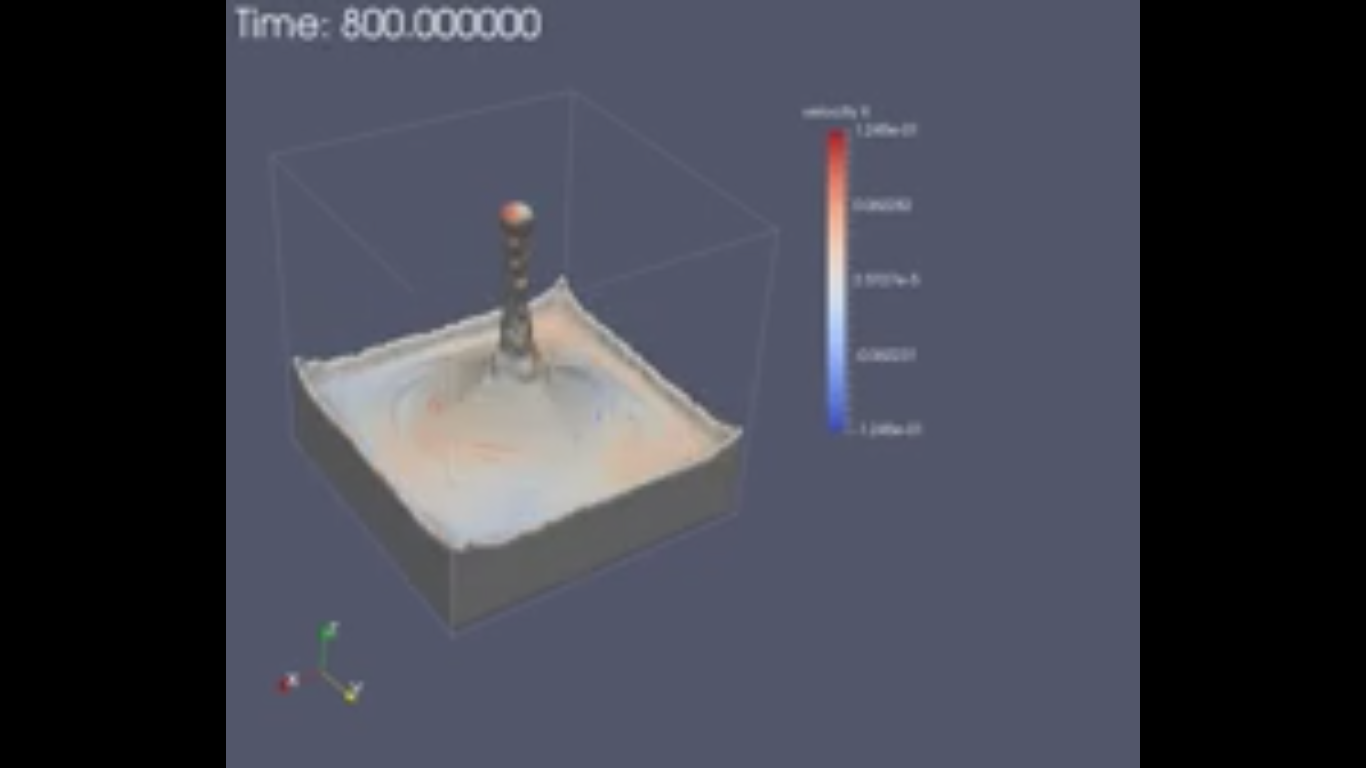
\includegraphics[width=1.0\linewidth]{drop/5.png}
\end{subfigure}
\begin{subfigure}{0.25\textwidth}
  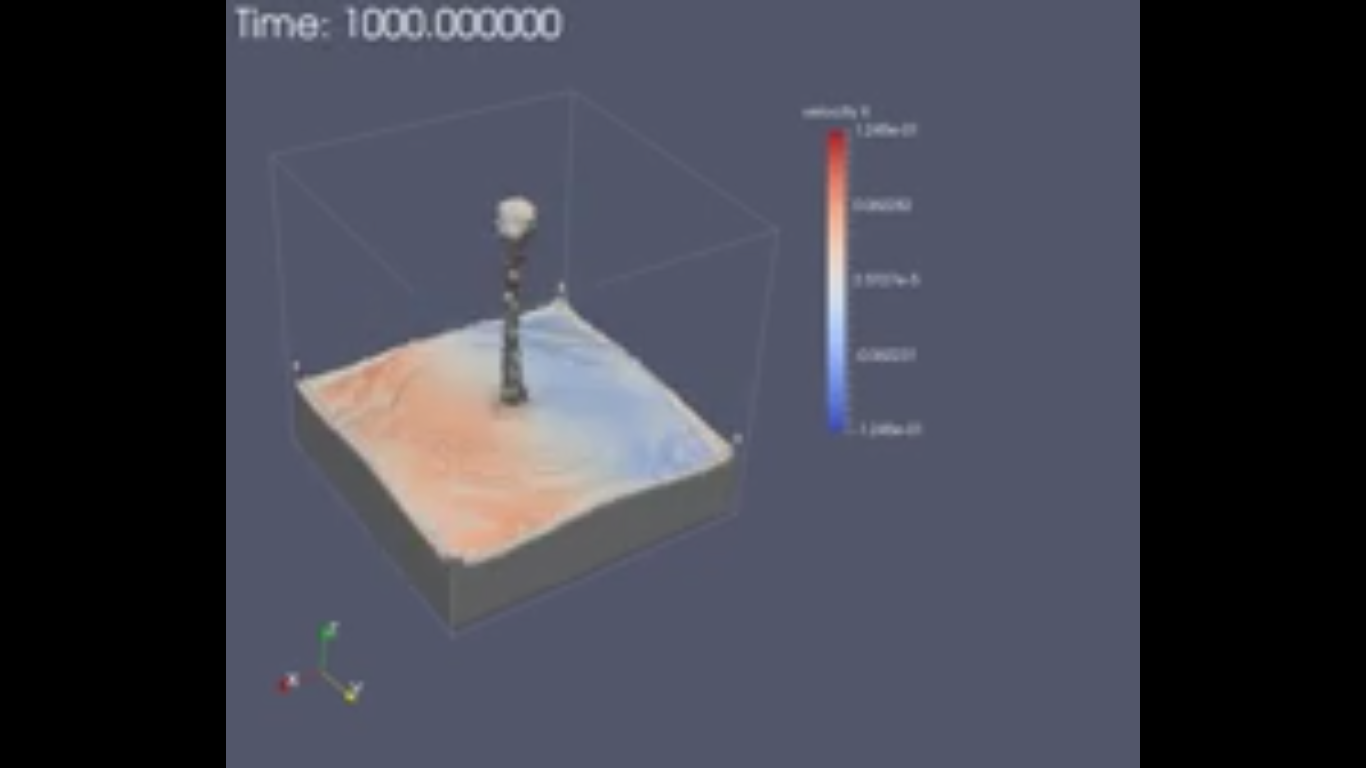
\includegraphics[width=1.0\linewidth]{drop/6.png}
\end{subfigure}
\centering
\begin{subfigure}{0.25\textwidth}
  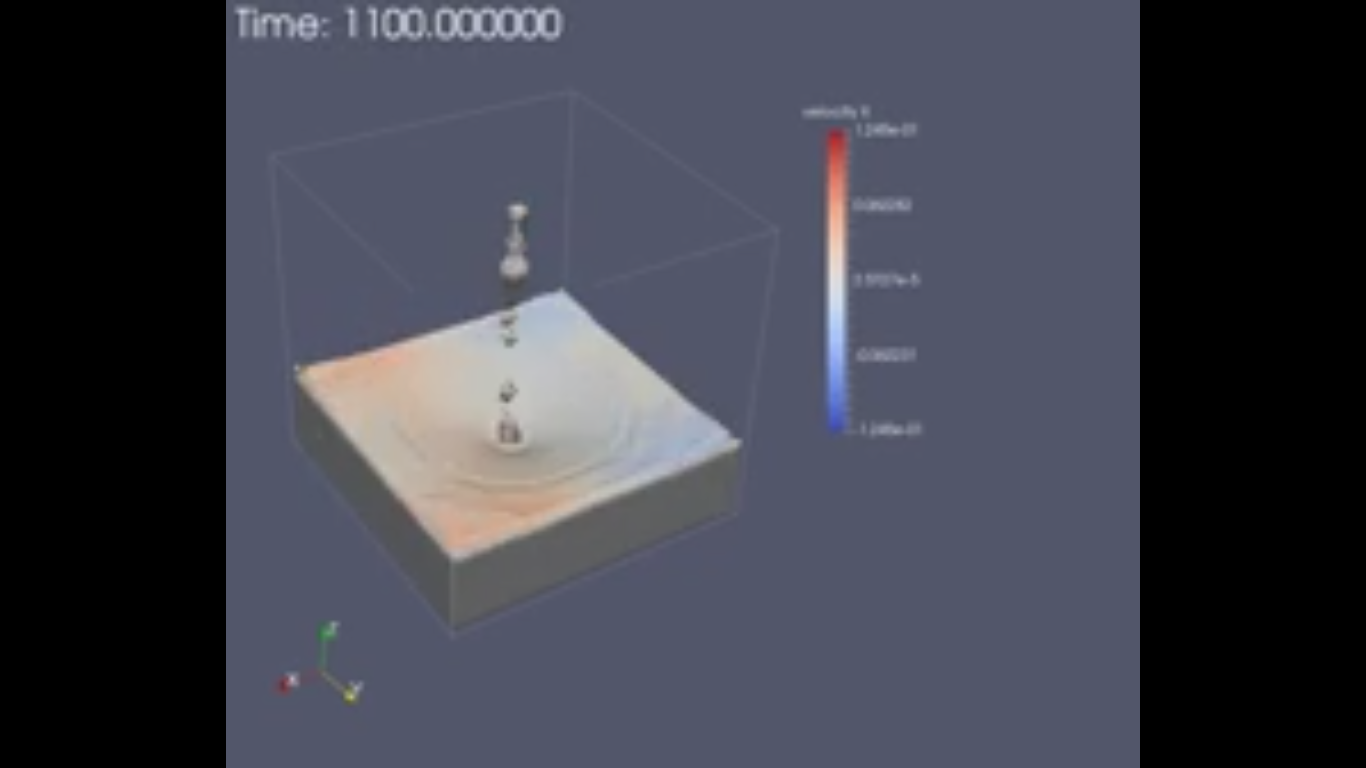
\includegraphics[width=1.0\linewidth]{drop/7.png}
\end{subfigure}%
\begin{subfigure}{0.25\textwidth}
  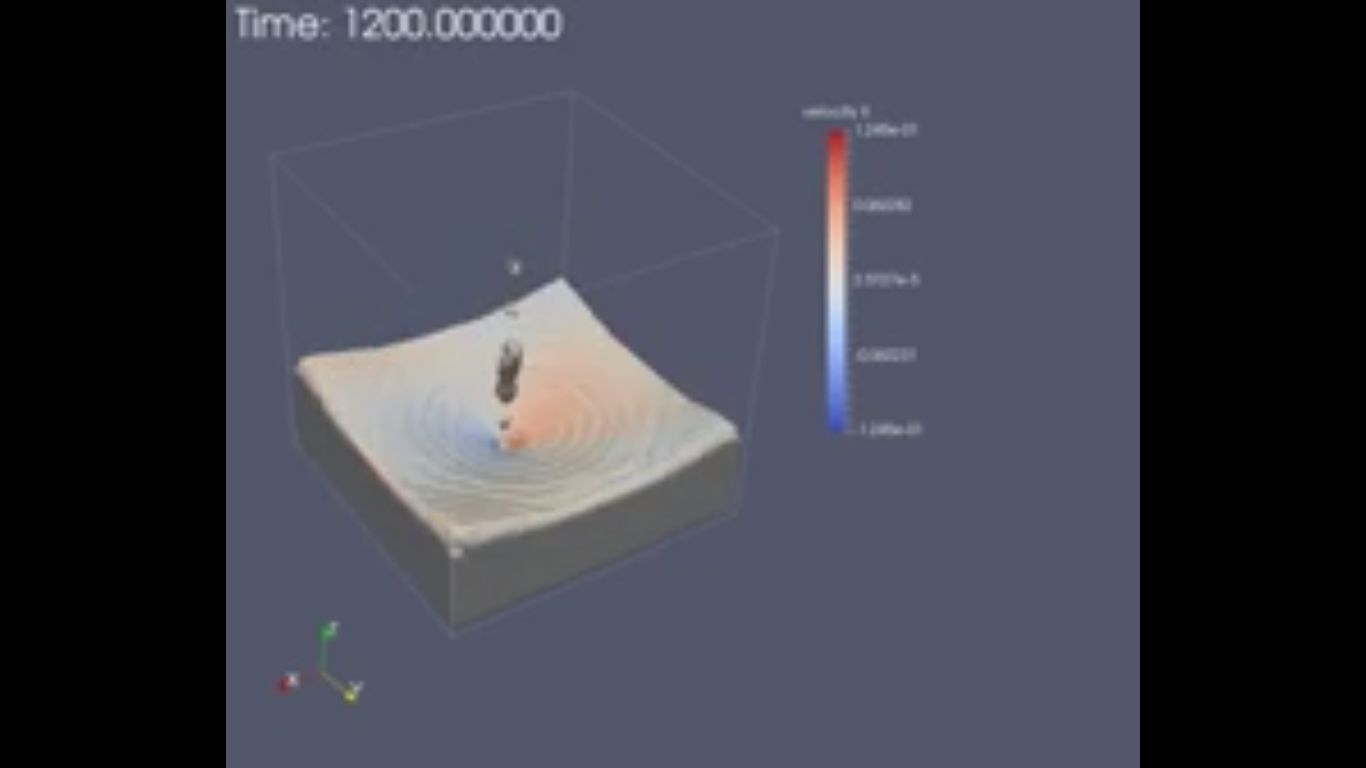
\includegraphics[width=1.0\linewidth]{drop/8.png}
\end{subfigure}
\begin{subfigure}{0.25\textwidth}
  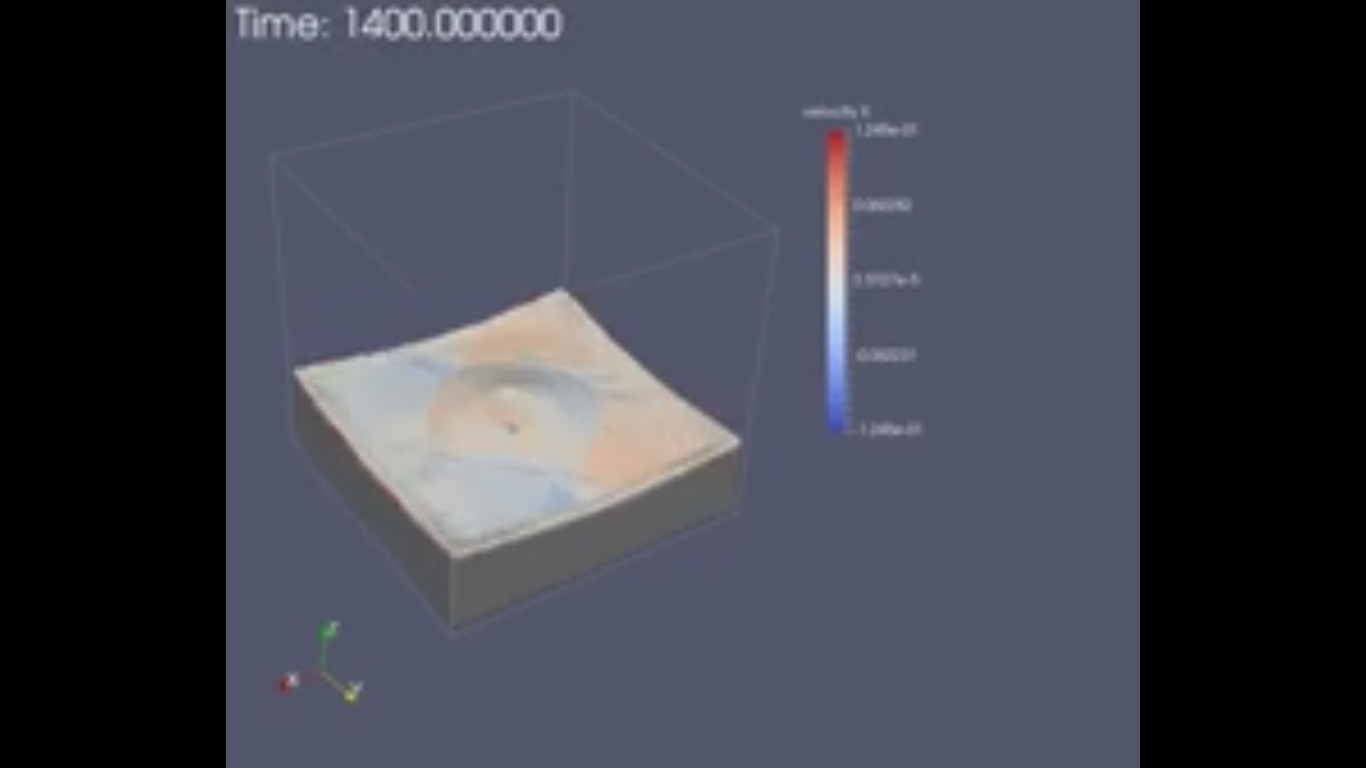
\includegraphics[width=1.0\linewidth]{drop/9.png}
\end{subfigure}
\caption{Falling Drop}
\label{fig:drop}
\end{figure}

\bibliographystyle{alpha}
\bibliography{refs}

\end{document}\grid



\grid
\grid
